\documentclass[12pt]{beamer}

\hypersetup{colorlinks=true,linkcolor=red}
\usetheme{default}
\usecolortheme{albatross}

\usepackage[utf8]{inputenc}
\usepackage[russian,english]{babel}
\usepackage[T2A]{fontenc}
\usepackage{hyperref}
\usepackage[final]{listings}
\usepackage{breakurl}
\usepackage{cite}
\usepackage{perpage}

\graphicspath{{img/}}

\def\Url\Breaks{\do\/\do-}
\lstset{
  frame=single,
  breaklines=true,
  basicstyle=\tiny,
  postbreak=\raisebox{0ex}{\ensuremath{\hookrightarrow\space}},
  numbers=left
}

\MakePerPage{footnote}

\title{Operating Systems}
\subtitle{OOO Execution and hardware assisted synchronization}
\author{Me}
\date{\today}

\begin{document}
  \begin{frame}
    \titlepage
  \end{frame}

  \begin{frame}[fragile]
\frametitle{Алгоритм Петерсона: то, что написали вы}
\begin{lstlisting}
int turn;
int claim[2];

void lock(int thread)
{
	const int other = (thread + 1) & 1;

	clain[thread] = 1;
	turn = other;

	while (claim[other] && turn != thread);
}

void unlock(int thread)
{
	claim[thread] = 0;
}
\end{lstlisting}
\end{frame}

\begin{frame}[fragile]
\frametitle{Алгоритм Петерсона: то, что уидел компилятор}
\begin{lstlisting}
.comm claim, 8

lock:
	/* eax = thread + 1 */
	leal	1(%rdi), %eax
	/* rdx = thread */
	movslq	%edi, %rdx
	/* claim[thread] = 1 */
	movl	$1, claim(,%rdx,4)
	/* eax = eax & 1, aka, eax = other */
	andl	$1, %eax

	/* rdx = other */
	movslq	%eax, %rdx

	/* check if claim[other] == 0 */
	movl	claim(,%rdx,4), %edx
	testl	%edx, %edx
	je	exit

	/* check if other == thread */
	cmpl	%eax, %edi
	je	exit

loop:	jmp	loop

exit:	ret
\end{lstlisting}
\end{frame}

\begin{frame}
\frametitle{Почему???}
\begin{itemize}
  \item Почему компилятор выкинул turn?
  \begin{itemize}
    \item Компилятор не увидел смысла в сохранении turn и удалил его.
  \end{itemize}
  \item Почему компилятор сравнивает other с thread?
  \begin{itemize}
    \item Компилятор выкинул turn, other - это значение, которое должно было
    лежать в turn.
  \end{itemize}
  \item Почему компилятор проверяет условия только один раз?
  \begin{itemize}
    \item Компиялтор не видит, что turn или claim могут измениться, а значит
    достаточно проверить их один раз и либо выйти либо зациклиться.
  \end{itemize}
\end{itemize}
\end{frame}

\begin{frame}
\frametitle{Компилятор виноват?}
\begin{itemize}
  \item Компилятор работает в терминах наблюдаемого поведения:
  \begin{itemize}
    \item компилятор может делать с вашей программой все что угодно, до тех пор
    пока наблюдаемое поведение сохраняется;
    \item компилятор хочет делать с вашей программой много чего, потому что он
    должен оптимизировать код.
  \end{itemize}
  \item Как сделать операции над данными частью наблюдаемого поведения?
  \begin{itemize}
    \item в языках C и C++ для этого есть ключевое слово \emph{volatile};
    \item компилятор воздерживается от многих оптимизаций кода работающего над
    volatile объектами.
  \end{itemize}
\end{itemize}
\end{frame}

\begin{frame}[fragile]
\frametitle{Оптимизации компилятора и volatile}
\begin{itemize}
  \item Пометив данные как volatile вы связываете компилятору руки везде, где
  вы используете volatile данные
  \begin{itemize}
    \item причем везде - и там где это важно и там где нет;
    \item есть ли более точечные средства ограничения фантазии компилятора?
    \item обычно они есть, но они зависят от компилятора.
  \end{itemize}
  \item Барьеры компиялтора:
  \begin{itemize}
    \item например, в gcc можно использовать такую конструкцию
\begin{lstlisting}
__asm__ volatile ("" : : : "memory")
\end{lstlisting}
  \end{itemize}
\end{itemize}
\end{frame}

\begin{frame}[fragile]
\frametitle{Алгоритм Петерсона с барьерами компиялтора}
\begin{lstlisting}
int turn;
int claim[2];

void lock(int thread)
{
	const int other = (thread + 1) & 1;

	claim[thread] = 1;
	__asm__ volatile ("" : : : "memory"); // order is important here
	turn = other;

	do {
		// reread claim and turn after every iteration
		__asm__ volatile ("" : : : "memory");
	} while (claim[other] && turn != thread);
}

void unlock(int thread)
{
	claim[thread] = 0;
}
\end{lstlisting}
\end{frame}

\begin{frame}
\frametitle{Замечания про volatile}
\begin{itemize}
  \item volatile не может являться средством синхронизации:
  \begin{itemize}
    \item volatile не дает никаких гарантий атомарности, т. е. работа с volatile
    переменными все еще не атомарна;
    \item стандарты C и C++ вводят такое понятие как \emph{точка следования},
    между двумя точками следования операциям компиялтору разрешено
    переупорядочивать обращения к volatile объектам;
    \item стандарты не определяют строго, что такое "обращение" к volatile
    объекту;
    \item компиялтор - не единственный источник переупорядочивания/оптимизаций,
    т. е. только компиялторных средств не достаточно.
  \end{itemize}
\end{itemize}
\end{frame}

  \begin{frame}
\frametitle{Многоуровневая организация памяти}
\begin{center}
  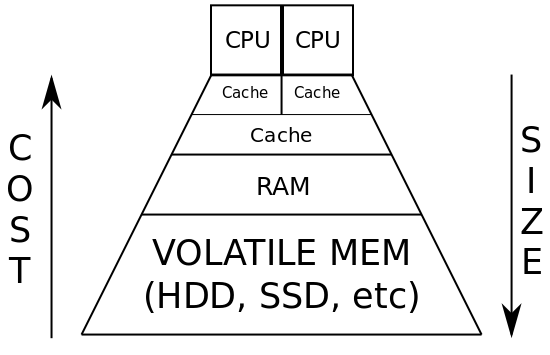
\includegraphics[width=0.6\linewidth]{hierarchy.png}
\end{center}
\begin{itemize}
  \item CPU очень быстрый, а память либо медленная либо дорогая
  \begin{itemize}
    \item поэтому приходится использовать несколько уровней памяти;
    \item чем ближе память к процессору, тем она быстрее и тем ее меньше;
  \end{itemize}
\end{itemize}
\end{frame}

\begin{frame}
\frametitle{Принцип локальности}
\begin{itemize}
  \item Временная локальность:
  \begin{itemize}
    \item когда программа обращается к одним и тем же данным в течение короткого
    интервала времени;
    \item пример: цикл считающий сумму элементов массива - переменная с
    результатом обновляется на каждый элемент массива.
  \end{itemize}
  \item Пространственная локальность:
  \begin{itemize}
    \item когда программа обращается к близким ячейкам памяти в течение
    короткого интервала времени;
    \item пример: цикл считающий сумму элементов массива - мы читаем элементы
    массива последовательно.
  \end{itemize}
  \item Зачастую, ваша программа не работает сразу со всеми петабайтами данных
  одновременно.
\end{itemize}
\end{frame}

\begin{frame}
\frametitle{Когерентность кешей}
\begin{itemize}
  \item CPU, зачастую, имеет свой собственный кеш:
  \begin{itemize}
    \item что если два CPU в своих кешах закеширвоали одну и ту же переменную?
    \item ничего плохого, пока копии идентичны;
    \item что если один из CPU решил обновить значение у себя в кеше?
    \item одна и та же переменная будет иметь разные значения для разных CPU.
  \end{itemize}
  \item Архитектуры, которые разрешают кешам "расходиться" называются
  некогерентными
  \begin{itemize}
    \item не менстрим.
  \end{itemize}
\end{itemize}
\end{frame}

\begin{frame}
\frametitle{Протоколы когерентности кешей}
\begin{itemize}
  \item Для обеспечения когерентности кеши могут обмениваться сообщениями
  \begin{itemize}
    \item CPU соединены между собой полноценной сетью;
    \item не такой как TCP/IP/Ethernet, но все еще полноценной.
  \end{itemize}
  \item Классы сообщений и как нужно на них реагировать - протокол когерентности
  кешей
  \begin{itemize}
    \item классический \emph{учебный} пример - протокол MESI.
  \end{itemize}
\end{itemize}
\end{frame}

\begin{frame}
\frametitle{Протокол MESI 1/3}
\begin{itemize}
  \item Каждая кеш-линия имеет одно из следующих состояний:
  \begin{itemize}
    \item M (Modified) - версия данных в кеш линии отличается от того, что
    хранится в памяти, а кроме того данный кеш является \emph{единственным}
    владельцем данных;
    \item E (Exclusive) - версия данных в кеш линии совпадает с тем, что
    хранится в памяти, и данный кеш \emph{единственный} владелец данных;
    \item S (Shared) - версия данных может находится в других кешах, и совпадает
    с тем, что хранится в памяти;
    \item I (Invalid) - кеш линия не хранит данных.
  \end{itemize}
\end{itemize}
\end{frame}

\begin{frame}
\frametitle{Протокол MESI 2/3}
\begin{itemize}
  \item Кеши и память обмениваются друг с другом сообщениями:
  \begin{itemize}
    \item мы считаем все сообщения широковещательными, т. е. каждый видит все
    сообщения.
  \end{itemize}
  \item Состояние кеш линии, обычно, меняется в ответ на получение сообщения.
  \item Modified может измениться в Exclusive, если процессор решил обновить
  версию в памяти
  \begin{itemize}
    \item кеш имеет ограниченный размер и когда-то мы должны из него что-то
    выбросить;
    \item если кеш хранит более новую версию чем память, то перед тем как
    выбрасить ее из кеша нужно обновить память;
    \item любую кеш линии в состоянии S или E можно спокойно выбрасывать из
    кеша.
  \end{itemize}
\end{itemize}
\end{frame}

\begin{frame}
\frametitle{Протокол MESI 3/3}
\begin{itemize}
  \item Типы сообщений:
  \begin{itemize}
    \item Read - у нас в кеше нет данных, мы хотим прочитать их из памяти или
    другого кеша;
    \item Read Response - ответ на запрос Read, вообще говоря, ответить может
    кто угодно, но мы будем считать, что отвечает всегда кеш, в котором есть
    данные или память, если кеша с новой версией данных не нашлось;
    \item Invalidate - заставить все кеши сбросить свою версию определенных
    данных;
    \item Invalidate Ack - подтверждение, что другие кеши сбросили свою версию
    данных, только получив подтверждение мы можем двигаться дальше;
    \item Read Invalidate - Read и Invalidate вместе, т. е. не только дайте мне
    данные, но еще и удалите их у себя.
  \end{itemize}
\end{itemize}
\end{frame}

\begin{frame}
\frametitle{Финальные замечания про когерентность кешей}
\begin{itemize}
  \item Фактически, чтобы обновить разделяемые данные необходимо быть их
  единственным владельцем:
  \begin{itemize}
    \item перед тем, как мы сможем обновить данные в кеше, кеш линия должна быть
    в состоянии E или M;
    \item запись в общие данные приводит к обмену сообщениями, ожиданию ответов
    и поэтому стоит дорого;
    \item нужно избегать записи в одну и ту же переменную с разных CPU, или
    ограничивать количество CPU пишущих в одну переменную;
    \item другими словами нужно избегать активной конкуренции (contention).
  \end{itemize}
\end{itemize}
\end{frame}

  \begin{frame}[fragile]
\frametitle{Теперь CPU виноват?}
\begin{columns}
  \begin{column}{0.35\linewidth}
    \begin{lstlisting}
#define barrier() \
  __asm__ volatile( "" \
	: \
	: \
	: "memory")

void foo(void)
{
  a = 1;
  barrier();
  b = 1;
}

void bar(void)
{
  while (b == 0) {
    barrier();
    continue;
  }
  barrier();
  assert(a == 1);
}
    \end{lstlisting}
  \end{column}
  \begin{column}{0.6\linewidth}
  \begin{itemize}
    \item Посмотрим на функцию bar:
    \begin{itemize}
      \item допустим переменная \emph{a} находится в кеше CPU, а переменная
      \emph{b} нет;
      \item т. е. чтение \emph{a} занимает много меньше времени, чем \emph{b};
      \item если CPU будет ждать пока завершится чтение \emph{b} ему придется
      остановиться;
      \item но у него уже есть \emph{a} и он \emph{не знает} о зависимости между
      ними, так может обработаем \emph{a} вперед?
    \end{itemize}
  \end{itemize}
  \end{column}
\end{columns}
\end{frame}


  \begin{frame}
  \begin{center}
  \Huge Q\&A
  \end{center}
  \end{frame}
\end{document}
